\documentclass{article}
\usepackage{graphicx} % Required for inserting images

\title{CTA200 Assignment 3}
\author{Shuo Chen}
\date{2026}

\begin{document}

\maketitle
\section{Question 1}
In this question, we determined the possible complex values of $c$ that do not cause the recursive relation
$$z_{i+1}=z_i^2+c$$
to diverge when provided with initial value $z_0=0$. The function defined for the equation was given a maximum number of iterations of $30$, and the criteria for divergence was if the value of $z^2>8$. Since the value of $c=x+iy$ is constrained by $x\in(-2,2)$ and $y\in(-2,2)$, a convergent $z$ would remain within the bounds
$$|z|^2=x^2+y^2\le 8$$
\begin{figure}[ht!]
    \centering
    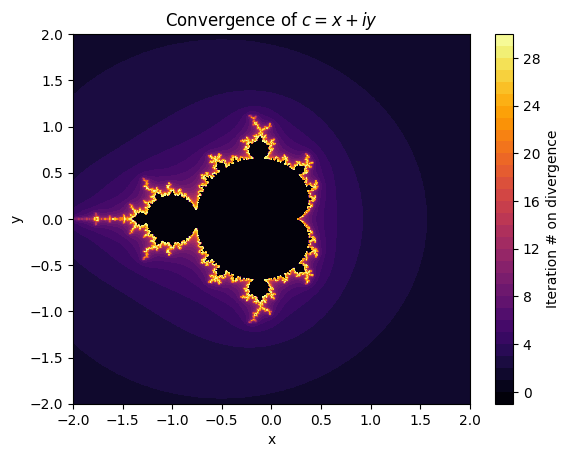
\includegraphics[width=0.7\linewidth]{mandelbrot.png}
    \caption{Regions where the recursive equation diverges or converges. Convergent values of $c$ have iteration number $-1$. (The darkest regions near the centre)}
    \label{q1_mandelbrot}
\end{figure}

If after 30 iterations the value of $z$ still satisfies this inequality, it classified as convergent. Otherwise, it is divergent. Plotting on a graph the values of $c$ that are convergent or divergent, we see on Figure \ref{q1_mandelbrot} that the complex numbers that lead to convergence form a fractal. Values that barely do not converge require many more iterations to diverge than values further away from the set, as shown by the bright regions close to the fractal.

\section{Question 2}
In this task, an imported function solve\_ivp from the scipy.integrate package was used to determine the behaviour of the amplitudes as a function of time. A separate function was written to determine the individual derivatives of each of the $X, Y, Z$ amplitudes, which was plugged into the IVP solver.

Compared to the graphs from the Lorenz paper, the time steps used here are different by 2 orders of magnitude, but the results are still very similar. The results for the amplitude of the $Y$ component is shown in Figure \ref{q2_lorenz1}.
\begin{figure}[ht]
    \centering
    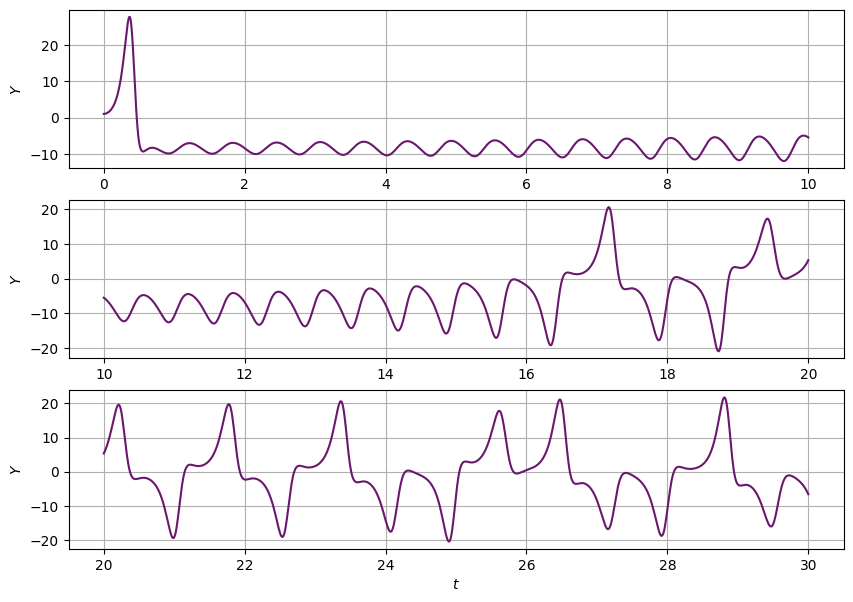
\includegraphics[width=0.9\linewidth]{Lorenz_1.png}
    \caption{Simulated results for initial values $W_0=(1,0,1)$. This matches with Lorenz' results in Figure 1 of their paper.}
    \label{q2_lorenz1}
\end{figure}

One key difference is the pattern in the last 1000 iterations (The bottom graph of Figure \ref{q2_lorenz1}) is slightly different to the one by Lorenz. This may be due to the difference in computational methods, which would cause some differences in the behaviour of the amplitude. However, the chaotic behaviour seen here still match the chaos found by Lorenz.\\[10 pt]

Changing the initial conditions by a factor of $10^{-8}$ causes the chaotic behaviour of the solution to diverge greatly from the original results. The distance between the new and old initial conditions is graphed in Figure \ref{q2_lorenzline}. Unlike the results obtained by Lorenz, the graph is stochastic and not a straight line, but taking the average values between $t=20$ and $t=40$, we can see that there is a relatively linear growth of the logarithm of distance, which does correlate with exponential growth.
\begin{figure}[ht]
    \centering
    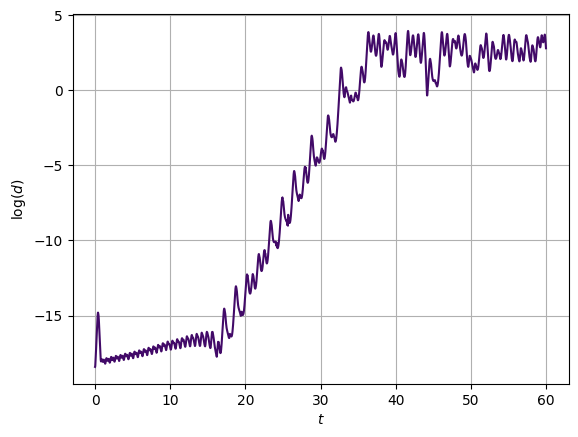
\includegraphics[width=0.7\linewidth]{Lorenz_line.png}
    \caption{Distance between ODE solutions with initial values $W_0$ and $W_0'=(0,1+10^{-8}, 0)$ as a function of time.}
    \label{q2_lorenzline}
\end{figure}

\end{document}
